\documentclass[tikz]{standalone}
\usetikzlibrary{automata,positioning}
\begin{document}

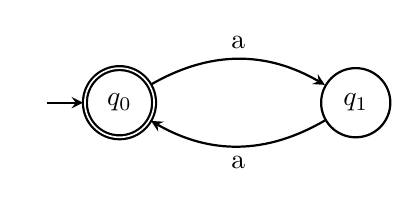
\begin{tikzpicture}[>=stealth,node distance=3cm,on grid,auto, thick, initial text=] 
  \node[state, initial, accepting] (q_0) {$q_0$};
  \node[state] (q_1) [right=of q_0] {$q_1$};

  \path[->]  (q_0) edge [bend left] node {a} (q_1)
  (q_1) edge [bend left] node {a} (q_0);
\end{tikzpicture}
\end{document}
